\documentclass{article}
\usepackage{scrextend}
\usepackage[utf8]{vietnam}
\usepackage{titling} 
\usepackage{setspace}
\usepackage[a4paper, total={170mm,257mm},left=25mm,right=25mm, top=20mm,]{geometry}
\usepackage{unicode-math}
\usepackage{amsfonts}
\usepackage{amsmath}
\DeclareMathOperator*{\argmax}{arg\,max}
\usepackage[symbol]{footmisc}
\makeatletter
\newcommand\footnoteref[1]{\protected@xdef\@thefnmark{\ref{#1}}\@footnotemark}
\makeatother
\usepackage{footnotehyper}
\usepackage{perpage} %the perpage package
\MakePerPage{footnote}

\usepackage{scrextend}
\title{\textbf{Dive into Deep Q-Network Algorithm\footnote[1]{This is our report for CS115 - Mathematics for Computer Science (Fall 2020) at University of Information Technology - Vietnam National University HCMC}}}
\setlength{\parindent}{0pt}
\usepackage{indentfirst}
\setlength{\parindent}{0pt}
\usepackage{ragged2e}
\usepackage[english]{babel}
\usepackage[square,numbers]{natbib}
\usepackage[colorlinks, citecolor = black, urlcolor = gray, bookmarks = false, hypertexnames = true ]{hyperref} 
\bibliographystyle{abbrvnat}
\author{
  \textbf{Ngoc-Tan Pham\footnotemark[2]}\\
  \small ngctn3701@gmail.com
  \and
  \textbf{Tri-Dzung Bui\footnotemark[2]}\\
   \small btrdung1621@gmail.com
  \and
  \textbf{An Khanh Vo\footnotemark[2]}\\
  \small vokhanhan25@gmail.com
  \footnotetext{Faculty of Computer Science, University of Information Technology, Vietnam National University HCMC}}
  
\date{December 2020}

\usepackage{graphicx}

\usepackage[ruled, lined, linesnumbered, commentsnumbered, longend]{algorithm2e}
\usepackage{xcolor}
\usepackage{mathtools}
\usepackage[]{algorithm2e}

\begin{document}

\maketitle

\begin{abstract}
\justifying 
\noindent 
    Deep Q-Network is an important algorithm, used to solve sequential decision making problems. It involves training a Deep Neural Network called a \textit{Deep Q-Network (DQN)}, to approximate a function associated with optimal decision making, the \textit{Q-function}. \textit{Deep Q-Network} has been reaching its peak by defeating former go champion - Lee Sedol, and became both famous and empirically successful all around the world in the field of Computer Science. Its theoretical foundation make it relatively difficult to understand completely, however, through the combination between \textit{Neural network} \cite{NeuralNetwork} and \textit{Q-Learning} \cite{QLearning}. In this work, we make our first attempt to theoretically understand the \textit{Deep Q-Network algorithm} \cite{ZDeepQLearn} from both algorithmic and mathematical perspectives. Besides, we shall take experiments to clarify the advantages of \textit{Deep Q-Network} in comparison with \textit{Double Deep Q-Network (Double DQN)} by means of detailed figures.
    \footnotetext[2]{Faculty of Computer Science, University of Information Technology -  Vietnam National University HCMC}
\end{abstract}


\section{Introduction}

\begin{flushleft} \justifying

Previously, computer scientists optimize decision-making problems by interacting with the environment and learning from the experiences, which in details, they have to find an optimal policy in the sense of maximizing the expected value of the total reward over any and all successive steps, starting from the current state. From this point of view, they came up with a brand new idea and they called it \textit{Q-Learning}. \textit{Q-Learning} is a model-free reinforcement learning algorithm to learn equality of actions telling an agent what action to take under what circumstances. It requires a non-model of the environment, or in another sayings, it uses model-free method to handle problems with stochastic transitions and rewards without requiring any adaptations. The main limitations for this kind of algorithm, however, are not having sufficient enough data sets to fast executive real world problems and having to learn a huge steps of very poor performance in simulation initially. This accidentally leads to the slowly and low-productively training process.\\ 

In such situations, computer scientists came up with another training method, which the agent had good online performance from the start of learning. They proceed pre-training agent so that it is capable of performing perfectly in the task from the start of learning, and then improving continually from its own self-generated data. They propose, in details, a new deep reinforcement learning algorithms, called \textit{Deep Q-Learning}. We can make it easy by considering it a method to leverage even very small amounts of demonstration data to massively accelerate learning. With this breakthrough in computer science, agents now achieve tremendous success in solving highly challenging problems, the game of Go, for instance, which we have mentioned above. In \textit{Deep Q-Network}, the value of policy functions is often represented as deep neural networks and the related deep learning techniques can be applied.

\end{flushleft}
\section{Background}
\subsection{Reinforcement learning}
Before starting, let imagine a gold digger. He works in a mine. He usually have to dig in different places each time. Once he digs a gold, he will get $100$ dollars. In an \textit{Markov decision processing} (MDP), the mine is the environment, the gold digger is the agent, $100$ dollar is the reward. Each time he goes through the mine or each time he digs a gold, we called it an action. Each step he goes, we called it the state. Our problem here is how that gold digger can achieve as much cumulative money as possible. In other words, it is the agent's goal to maximize the cumulative rewards.\\

\subsubsection*{Key notion:}
The figure below shows us a visualization of MDP's cycle:
\begin{figure}[h!]
\centering
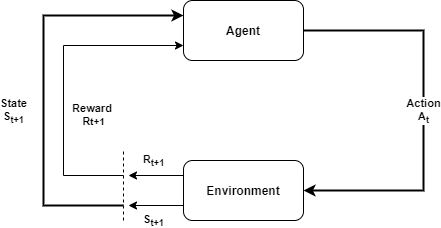
\includegraphics[scale=0.5]{CycleOfTheAgent.png}
\caption{Markov decision process' cycle}
\end{figure}

Verbally, we can say:
\begin{itemize}
    \item \textbf{Step 1}: At time \textbf{$t$}, the environment has the state of \textbf{$S_t$}
    \item \textbf{Step 2}: The agent decides which action \textbf{$A_t$} to take next, based on current state
    \item \textbf{Step 3}: The environment will change its state, from \textbf{${S_t}$} to \textbf{$S_{t+1}$}. The agent will achieve the reward \textbf{$R_{t+1}$} afterwards
    \item \textbf{Step 4}: We assign $t$ by $t + 1$, then we return to \textit{step 1}
\end{itemize}
At \textit{step $2$} above, the agent decides to choose the action $A_t$ based on the transition probabilities.\\
Let denote this probability by:\\
\begin{equation}
\label{probability}
p(s', r \mid s, a) = \mathbb{P}\{S_t = s', R_t = r \mid S_{t-1} = s, A_{t-1} = a\} \nonumber
\end{equation}
The $p$ function returns the transition probability from state $s$ to $s'$ after doing the action $A$ and get the reward of $R$. We assign $\mathbb{P}$ as the probability from now on.\\

\textit{Expected return} is used to measure either how good a state is or how worth an action will be. \textit{Future reward}, or \textit{return}, is the sum of the \textit{discounted reward} multiplied by the reward at time $t$.
\begin{equation}
G_t = R_{t+1} + \gamma R_{t+2} + ... = \sum_{k = 0}^{\infty}\gamma^kR_{t+k+1}  
\end{equation}

The \textit{discounted factor}, or the $\gamma \in \left[0; 1\right]$, penalizes the rewards in the future. We need that formula to avoid divergence and result in infinity loop. In other hand, this can be seen as the uncertainty for future reward, e.g., weather forecast, and the further the reward is, the less immediate benefit we achieve.\\

We can transform $(\ref{probability})$ into:
\begin{align} 
G_t &= R_{t+1} + \gamma R_{t + 2}  + \gamma^2 R_{t + 3} + \gamma^4 R_{t + 4} + ...  \nonumber \\
    &= R_{t + 1} + \gamma (R_{t + 2} + \gamma R_{t + 3} + \gamma^2 R_{t + 4} + ...) \nonumber \\
    &= R_{t + 1} + \gamma G_{t + 1} \nonumber 
\end{align}

This transformation shows us the correlation between continuous time steps
\begin{align}
\label{policy}
V_{\pi}(s)  &= \mathbb{E}_{\pi}\left[G_{t} \mid S_{t} = s\right] \nonumber \\
            &= \mathbb{E}_{\pi}\left[\sum_{k = 0}^{\infty} \gamma^k R_{t+k+1} \mid S_t = s\right]
\end{align}
Equation $(\ref{policy})$ can be understood as the value of state $S$($v_\pi$) followed by policy $\pi$ is the expected return from state $s$ at time $t$ followed by policy $\pi$ thereafter.

\begin{align}
Q_{\pi}(s, a)   &= \mathbb{E}_{\pi}\left[G_t \mid S_t = s, A_t = a \right] \nonumber \\
                &= \mathbb{E}_{\pi}\left[\sum_{k = 0}^{\infty} \gamma^k R_{t+k+1} \mid S_t = s, A_t = a\right]
\end{align}
\\
\textit{Q-function}, denoted by \textit{action-value function} $Q_{\pi}$, has the return result for any given actions-states pair called \textit{Q-value}. \textit{Q-function} can be understood as the value of action $a$ in state $s$ followed by policy $\pi$, calculated by expected return from the beginning of state $s$ at time $t$ taking action $a$ followed by policy $\pi$ thereafter.

\begin{equation}
    V_{\pi}(s) = \sum_{a \in A} Q_{\pi}(s, a)\pi(a \mid s) \nonumber 
\end{equation}
Besides, since we follow policy $\pi$, we can get \textit{state value} by multiplying probability distribution of possible actions at a state by \textit{Q-values}.

\begin{equation}
    A_{\pi}(s, a) = Q_{\pi}(s, a) - V_{\pi}(s) \nonumber
\end{equation}
Should we take the difference between \textit{Q-value} and \textit{state value}, we shall get a new value, which is \textit{A-value}, used to recognize how precious an acted action at a certain state is.

\begin{equation}
\label{Optimal state value function}
V_{*}(s) = \underset{\pi}{\max}v_{\pi}(s) \textrm{ for all s $\in$ \textbf{S}}
\end{equation}
The \textit{optimal state-value function} $V_{*}$ shows us the \textit{maximum expected benefit} we can achieve by any policy $\pi$ for each state.

\begin{equation}
\label{Optimal Q-function}
Q_{*}(s, a) = \underset{\pi}{\max}Q_{\pi}(s, a) \textrm{ for all s $\in$ \textbf{S} and for all a $\in$ \textbf{A}(s)}
\end{equation}
The \textit{optimal Q-function} $Q_{*}$ brings us the \textit{maximum expected value} by any given policy for each possible state - action pair.

From $(\ref{Optimal state value function})$ and $(\ref{Optimal Q-function})$, we get the optimal-value function:
\begin{align}
\pi_{*} &= \underset{\pi}{\argmax } \textrm{ $V_{\pi}(s)$ } \nonumber   \\
        &= \underset{\pi}{\argmax } \textrm{ $Q_{\pi}(s, a)$} \nonumber
\end{align}


\subsubsection*{Bellman Equation}
Bellman equation is a necessary condition for optimizing associated with mathematical optimizing method, called \textit{dynamic programming}. It is a set of equations to analyze the value functions into the sum of immediate rewards and future discounted values. This leads to dividing optimized problems into a series of simpler sub-problems.

\begin{align}
    Q(s, a) &= \mathbb{E}[R_{t+1} + \gamma V(S_{t+1}) \mid S_t, A_t = a ]
    \nonumber \\
            &= \mathbb{E}[R_{t+1} + \gamma \mathbb{E}_{a \stackrel{}{\sim}\pi}Q(S_{t+1}, a) \mid S_t = s, A_t = a]
    \nonumber \\
    \nonumber \\
    V(s)    &= \mathbb{E}[G_t \mid S_t = s] \nonumber \\
            &= \mathbb{E}[R_{t+1} + \gamma R_{t+2} + \gamma^2 R_{t+3} + ... \mid S_t = s] \nonumber \\
            &= \mathbb{E}[R_{t+1} + \gamma(R_{t+2} + \gamma R_{t+3} + ... ) \mid S_t = s] \nonumber \\
            &= \mathbb{E}[R_{t+1} + \gamma G_{t+1} \mid S_t = s] \nonumber\\
            &= \mathbb{E}[R_{t+1} + \gamma V(S_{t+1}) \mid S_t = s] \nonumber   
\end{align}

\newpage 

\begin{figure}[h!]
\centering
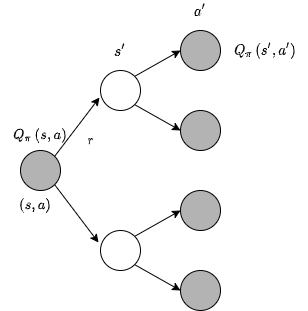
\includegraphics[scale=0.5]{BellmanTreeBuilding.png}
\caption{Bellman tree-building.}
\end{figure}

Geometrically, the Bellman tree-building process can transform equations into state-value functions and action-value functions. As we reach further, we can extend the tree as we mentioned before, according to policy $\pi$

\begin{align}
    Q_{*}(s, a) = \mathbb{E}[R_{t+1} + \gamma \underset{a'}{\max}Q_{*}(s', a') \nonumber]
\end{align}
The above equation is called \textit{Bellman optimality equation} for $Q_{*}$. This equation can be understood as the \textit{Q-value} is the expected reward $R_{t+1}$ we achieve when executing action $a$ at state $s$, plus the \textit{maximum expected discounted return} that can be achieved from any possible next state-action pair $(s', a')$. Since the agent is following an optimal policy, the state $s'$ will be the state from which the next best action $a'$ will be executed at time $t+1$.\\
When we have $Q_{*}$, we can identify the optimal policy. It is due to the fact that for any given state $s$, the \textit{reinforcement learning algorithm} can find action $a$ to maximize $Q_{*}(s, a)$.
% Since our agent follows an optimal policy $\pi_{*}$

\subsection{Q-learning}
\textit{Q-learning} is a model-free reinforcement learning algorithm to learn the quality of action $a$ to tell the agent which actions to execute at a certain state $s$. It does not require a model of a certain environment. It can handle dynamically environmental problems and achieve rewards without any adaptations. The development of \textit{Q-learning} is a breakthrough in early days of reinforcement learning.\\



The interesting point in \textit{Q-learning} is the independence of the current policy to choose the second action $a_{t+1}$. It, essentially, estimates $Q_{*}$ among the best \textit{Q-values}, but it does not matter which action leads to this maximum \textit{Q-value} and in the next step, this algorithm does not have to follow that policy.

\subsubsection*{Updating the Q-Value}

\newcommand\mycommfont[1]{\small\ttfamily\textcolor{blue}{#1}}
\SetCommentSty{mycommfont}


\begin{algorithm} 
    $t = 0$
    
    \While{$t \leftarrow 0$ not converged}{
        \State At time step $t$, we pick the action according to \textit{Q values},  $A_{t} = \textbf{argmax}_{a \in A} Q(S_{t}, a)$ and $\epsilon$ - greedy is commonly applied.
       
        \State After applying action $A_{t}$, we observe reward $R_{t+1}$ and get into the next state $S_{t+1}$.
          
        \State Update the Q-value function: 
        \State $Q(S_{t}, A_{t}) \leftarrow Q(S_{t}, A_{t}) + \alpha(R_{t+1} + \gamma \textbf{max}_{a \inA}Q(S_{t+1}, a) - Q(S_{t}, A_{t}))$
        
        \State $t = t + 1$
    }
    \Return{$Q$}
    \caption{Updating the Q-value}
\end{algorithm}


We want to create a \textit{Q-value} for action-state pair as close to the right hand side of the \textit{Bellman equation} as possible to make \textit{Q-value} converge on optimal \textit{Q-value} $Q_{*}$. Essentially, this can be made by iterating comparison the loss between \textit{Q-value} and the optimal Q-value $Q_{*}$ for each state-action pair. We update \textit{Q-value} over and over every time we meet this same state-action pair so as to reduce the loss, after that.

\begin{align}
    Loss &= Q_{*}(s, a) - Q(s, a) \nonumber \\
         &= \mathbb{E}\left[R_{t+1} + \gamma \underset{a'}{\max}Q_{*}(s', a')\right] - \mathbb{E}\left[\sum_{k=0}^{\infty} \gamma^kR_{t+k+1}\right]
\end{align}

We have the equation to calculate the new \textit{Q-value} for new state-action pair $(s, a)$ at time $t$:
\begin{equation} 
Q_{new}\left( s,a\right) =\left( 1-\alpha \right) ~\underset{\text{old value} }{\underbrace{Q\left( s,a\right) }\rule[-0.05in]{0in}{0.2in} \rule[-0.05in]{0in}{0.2in}\rule[-0.1in]{0in}{0.3in}}+\alpha \overset{\text{ learned value}}{\overbrace{\left(R_{t+1}+\gamma \max_{a^{^{\prime }}}Q\left( s^{\prime },a^{\prime }\right) \right) }} 
\end{equation}

Our new \textit{Q-value} is equal to a weighted sum of our old value and the learned value. In the first time, the old value is assigned to $0$ and the agent experiences this particular state-action pair. Then, we multiply the old value by $1 - \alpha$.\\

The \textit{learning rate} $\alpha$ is a real number between $0$ and $1$. It can be thought as how quickly the agent changes to abandon the previous \textit{Q-value} in \textit{Q-table} for a given state-action pair to perceive the new \textit{Q-value}.\\

Our \textit{learned value} is the reward from which our agent achieves moving right from the starting state, plus with the discounted estimate of future \textit{optimal Q-value} for the next state-action pair $(s', a')$ at time $t + 1$. We afterward multiply all the learned value with our learning rate $\alpha$.\\

Our newly calculated \textit{Q-value} will be stored in our \textit{Q-table} for this particular state-action pair, noticeably.\\

We have completed the single time step. Not until the end of episode will this process happen continuously. Once \textit{Q-function} converges on the \textit{optimal Q-function}, we receive the \textit{optimal policy}.

\section{Deep Q-Network}
Theoretically, we can store $Q_{*}$ for every state-action pair in \textit{Q-learning} into an enormous table. This can make the storage space in computer infeasibly, however, when the number of state-action pairs become gigantic. Thus, we shall find a new method to create a specific function for approximating the Q-value. Luckily, we are in the spring of the advances in deep learning techniques, which enable us to apply \textit{neural network} \cite{NeuralNetwork} into this case. This combination of deep learning of reinforcement learning is the significant discovery, and this combination is known as \textit{Deep Q-network} (DQN). Ideally, we can use a neural network with current state $s$ as input layer and the execute action as output layer instead of using an \textit{Q-table} to store huge state-action pairs as in \textit{Q-learning}.\\


% \begin{algorithm} 
    
%     Initialize replay memory $D$ to capacity $N$
    
%     Initialize action-value function $Q$ with random weights $\theta$
    
%     Initialize target action-value function $\hat{Q}$ with weights $\theta^{-} = \theta$
    
%     \For{$episode \leftarrow 1$ \KwTo $M$}{
%         Initialize sequence $s_{1} = \{ x_{1} \}$ and preprocessed sequence $\phi_{1} = \phi\left(s_{1}\right)$
%         \For{$t \leftarrow 1$ \KwTo $T$}{ 
%             With probability $\epsilon$ select a random action $a_{t}$ otherwise select $a_{t} = \underset{a}{\argmax} Q \left( \phi \left(s_t \right), a, \theta \right)$
            
%             Execute action $a_{t}$ in emulator and observe reward $r_{t}$ and image $x_{t+1}$
            
%             Set $S_{t+1} = S, a_{t}, x_{t+1}$ and preprocess $\phi_{t+1} = \phi\left(s_{t+1}\right)$
            
%             Store transition $\left( \phi_{t}, a_{t}, r_{t}, \phi_{t+1} \right)$ in $D$
            
%             Set $y_{i}: $
            
%             \If {episode terminates at step $j+1$}{
%                     $y_{i} = r_{j}$ 
%             }
%             \Else{
%                 $y_{i} = r_{j} + \gamma \textbf{max} _{a'}\hat{Q}\left(\theta_{j+1}, a'; \theta^{-} \right)$  
%             }
            
%             Perform a gradient descent step on ${\left(\gamma_{i} - Q\left(\theta_{j}, a_{j}; \theta \right)\right)}^{2} $ with respect to the network parameters $\theta$
            
%             Every $C$ steps reset $\hat{Q} = Q$
%         }
%     }
%     \caption{Deep Q Network}
% \end{algorithm}

Unfortunately, \textit{Deep reinforcement learning} also get into a variety of trouble. Reinforcement learning becomes more unstable when neural network is used to represent action value. Training a neural network requires such a great deal of data, but even if we get such an amount, it is not guaranteed neural network will converge on the optimal value function. In practice, there are conditions in which network's weights might be either diverged or oscillate due to the high correlation between actions and values.\\

It is \textit{experience replay} and \textit{target network} that DQN uses to stablize and improve significantly the training process.
\subsection*{Experience replay}
In DQN, we often use the technique, known as \textit{experience replay}. By this means, we can store the experience of our agent at each time step in our data set, or can be denoted as \textit{replay memory}. We express the experience at time $t$ as tuple $e_t$:

$$
e_t = (s_t, a_t, r_{t+1}, s_{t+1})
$$

All the experience at one time step in all episodes are all stored in \textit{replay memory}. In practice, our \textit{replay memory} has its own limitation, nevertheless. Thus, we are able to store \textbf{\textit{N}} last experience. \\

In this \textit{replay memory data set}, we retrieve random samples for training our neural network. The action of experience collecting and experience sample extracting from stored replay memory is called \textit{experience replay}. Our main reason for using replay memory is to break the correlate relation between continuous samples. Only if our neural network learns from continuous experience as they occurred sequentially in the environment do our samples get the highly correlate relation, which will lead to the inefficiency in learning.

\subsubsection*{Target Network}
Bellman equation provides us the value of $Q(s, a)$ via $Q(s', a')$. There is just one step among $s$ and $s'$, which leads to its high correlation between them. This is also a barrier and neural network will get difficulty in distinguishing them, as the result.\\

$Q(s, a)$ is as close as our desired output once we update neural network's parameters, we can indirectly change the parameters created for $Q(s', a')$ and those close by states. This accidentally leads to unstable neural network's training process.\\

To make our training process more stable, there is a technique called \textit{target network}. Through which, we can keep the neural network and use it for $Q(s', a')$ value in Bellman equation.\\

Q-value, which is predicted in our copy of Q-network, is called \textit{target network}. It will be used to backpropagate through and train the main Q-network. The importance which needs to be clarify is the untrained neural network's parameters, but they will be synchronized periodly with the main Q-network's parameters. The idea of using Q-value of target network to train main Q-network will increase the stability in training process.
\subsubsection*{Deep Q Network}
There are 2 main interleaved phases in Deep Q Network. One is we sample environment by means of taking actions and storing the observed experienced tuples in a replay memory. The another is we take a small batch of the tuple from the memory randomly, and learn from those batches through SGD to update steps \cite{SGD}. \\

Those 2 phases do not depend directly to each other and we can sample our data through many steps, and then one learning step, or even many learning steps with many random batches. In practice, we can not executive learning step immediately. Not until tuples of experience are not sufficient in replay memory $\mathfrak{D}$ will we have to execute.

\begin{algorithm} 
    Initialize network $Q$, target network $\hat{Q}$, experience replay memory $D$
    
    Initialize the Agent to interact with the Environment
    
    \While{not converged} 
    {
        $\epsilon \leftarrow$ setting new epsilon with $\epsilon-decay$
        
        Choose an action a from state $s$ using policy $\epsilon-greedy\left(Q\right)$
        
        Agent takes action $a$, observe reward $r$, and next state $s'$
        
        Store transition $\left(s, a, r, s', done \right)$ in the experience replay memory $D$
        
        \If{enough experiences in D}
        {
            Sample a random minibatch of $N$ transitions from $D$
            
            \For {every transition $\left(s_i, a_i, r_i, s_i', done_i\right)$}
            {
                \eIf{$done_i$}{$y_i = r_i$}{
                    $y_i = r_i + \gamma max_{a' \in A}\hat{Q}\left(s_i', a_'\right)$}
            }
            
            Calculate the loss $\mathcal{L} = 1/N \sum^{N-1}_{i=0}\left(Q\left(s_i, a_i\right) - y_i\right)^2$
            
            Update $Q$ using the SGD algorithm by minimizing the loss $\mathcal{L}$
            
            Every C steps, copy weights from $Q$ to $\hat{Q}$
        }
    }
    \caption{Deep Q Network Algorithm}
\end{algorithm}

We will intialize our main Q-network and target network, at first, and initilize empty replay memory $\mathfrak{D}$. Since we have to notice is the finity of our memory, we are able to use pseudo code circular queue to store $\mathfrak{N}$ near experience tuple. We will also initialize the agent, which will interact with the environment.\\

One noticable thing is that we will not clear our memory after episodes, which leads to our recall and mass memory building from episodes. This data map is what maps our algorithmic installation.\\

Our \textit{loss function} looks like:
\begin{equation}
    \mathcal{L}\left(\theta\right) = \mathbb{E}_{(s, a, r, s') \sim U(\mathfrak{D})} \Big[ \big( r + \gamma \max_{a'} Q(s', a'; \theta^{-}) - Q(s, a; \theta) \big)^2 \Big]
\end{equation}

in which $U(D)$ is the uniform distribution on replay memory $\mathfrak{D}$ and $\theta^{-}$ is the parameter of target Q-network.\\

\subsection*{Double Deep Q-Network}
We have discussed about basic \textit{Q-Learning} and \textit{Deep Q-Network} above. 
\subsubsection*{Motivation}
DQN is proposed to solve overestimation of Q-value in vanilla Q-Learning.\\

In vanilla Q-learning, the optimal policy of agent is always choosing the best action in every given action. The theory behind this idea is which the best action has the largest estimated Q-value. Nevertheless, our agent does not know anything about the environment, at the beginning, it has to estimate $Q(s, a)$ and update at each loop through. Such Q-values have a huge noise and at no times will we make sure whether the action with maximum estimated Q-values is the really dominated.\\

Unfortunately, the best action tends to have smaller Q-values opposed to the non-optimal one's in most of the cases. According to the optimal policy of vanilla Q-learning, the agent has a tendancy of take the non-optimal action in any given states, just for the the maximum Q-value. This problem is termed as \textit{overestimations of Q-value}.\\

When such problem happens, noises from estimated Q-values shall the big causes for \textit{positive biases} in update process. Consequently, learning process becomes sophisticated and messy.\\

Because of the noisy of current $Q(s, a)$ used to estimate the best $Q(s, a)$, \textit{positive biases} happen. The difference between the best $Q(s, a)$ and the current one in \textit{loss function} is also messy and contains positive biases, which are happened by different noises. Positive biases impact a high volume in the updating process
\begin{align}
    Loss &= Q_{*}\left(s, a\right) - Q\left(s, a\right) \nonumber \\
    Q_{*}\left(s, a\right) &= R_{t+1} + \gamma \underset{a'}{\max}Q_{*}\left(s', a'\right) \nonumber \\
    Q_{new}\left( s,a\right) &=\left( 1-\alpha \right) Q\left( s,a\right)  +\alpha {{\left(R_{t+1}+\gamma \max_{a^{^{\prime }}}Q\left( s^{\prime },a^{\prime }\right) \right) }}\nonumber 
\end{align}

More specifically, shall the noises of all Q-values have the \textit{uniform distribution} (Q-values have are equally overestimated), overestimation is not the problem since those noises do not affect to the difference between $Q(s^{\prime}, a)$ and $Q(s, a)$. This is originated from H. van Hasselt 2015 \cite{DQL}
\subsubsection*{Double Q-Learning}
\textit{Double Q-Learning} uses 2 different action-value functions, $Q$ and $Q'$ are estimators. Even if noises are noisy, they are still viewed as uniform distribution. That is, this algorithm solves the problem of estimations of action values.\\

The update procedure is different slightly in comparison to the basic one:\\

\textit{Basic Q-Learning:}
\begin{align}
   Q_{\left(s,a\right)} &= \left( 1-\alpha \right) Q\left( s,a\right)  +\alpha {{\left(R_{t+1}+\gamma \max_{a^{^{\prime }}}Q\left( s^{\prime },a^{\prime }\right) \right) }}\nonumber
\end{align}
\textit{Double Q-Learning:}
\begin{align}
   Q_{\left(s,a\right)} &= \left( 1-\alpha \right) Q\left( s,a\right)  +\alpha {{\left[R_{t+1}+\gamma Q'\left( s^{\prime }, \underset{a'}{\max}(s', a')\right) \right] }}\nonumber 
\end{align}
\textit{Q-function} is used to choose the best action $a$ with maximum Q-value of the next state.

\textit{$Q^{ \prime}$-function} is used to calculate the expected Q-value by using the chosen action $a$ above.

We update \textit{Q-function} by using expected Q-value of \textit{$Q^{\prime}$-function}


\begin{algorithm} 
    \SetAlgoLined
    Initialize $Q^A, Q^B, s$
    
    \Repeat{}
    {
        Choose $a$, based on $Q^A\left(s, .\right)$ and $Q^A\left(s, .\right)$, observe $r, s'$
        
        Choose (e.g. random) either UPDATE(A) or UPDATE(B)
        
        \If{UPDATE(A)}
        { 
            Define $a^*$ = $argmax_a Q^A\left(s', a\right)$
            $Q^A\left(s, a\right) \leftarrow Q^A\left(s, a\right) + \alpha\left(s, a\right)\left(r + \gamma Q^B\left(s', a^*\right) - Q^A\left(s, a\right)\right)$
        }
        \Else
        {
            Define $b^*$ = $argmax_b Q^B\left(s', a\right)$
            $Q^B\left(s, a\right) \leftarrow Q^B\left(s, a\right) + \alpha\left(s, a\right)\left(r + \gamma Q^A\left(s', a^*\right) - Q^B\left(s, a\right)\right)$
        }
        
        $s$ $\leftarrow$ $s'$
    }
    \caption{Double Q-learning}
\end{algorithm}


Nevertheless, this method also have the same drawbacks as Q-learning for its tabular way. We shall resolve this problem with deep neural network.
\subsubsection*{Double Deep Q-Network}
Inspired by Double Q-Learning, Double DQN splits \textit{deep neural network} in DQN into 2 seperation: \textit{Deep Q-Network} and \textit{target network}. In DQN, the target Q-Network selects and evaluates every action resulting in an overestimation of Q value. To resolve this issue, \textbf{DDQN proposes to use the Q-Network to choose the action and use the target Q-Network to evaluate the action}. In details:
\begin{enumerate}
    \item Deep Q Network chooses the best action $a$ with maximum Q-value of next state.
    \item Target network uses to evaluate Q-value with the selected action $a$ above
    \item Update Q-value of Deep Q-Network based on evaluated Q-value from target network
    \item Update target network's parameters based on deep Q network's parameters in each iteration
    \item Update deep Q network's parameters with \textit{Adam optimizer}
\end{enumerate}

\begin{algorithm} 
    Initialize primary network $Q_{\theta}$, target network $Q_{\theta^{\prime}}$, replay buffer $D$, $\tau \ll 1$
    
    \For{each environment step}
    {
        \For{each environment step}
        { 
            Observe state $s_t$ and select $a_t \sim \pi \left(a_t, s_t\right)$
            
            Execute $a_t$ and observe next state $s_{t+1}$ and reward $r_t = R\left(s_t, a_t\right)$
            
            Store $\left(s_t, a_t, r_t, s_{t+1}\right)$ in replay buffer D
        }
        \For{each update step}
        {
            sample $e_{t} = \left(s_t, a_t, r_t, s_{t+1}\right) \sim D$
            
            Compute target $Q$ value:
                $Q^*\left(s_t, a_t\right) \approx r_t + \gamma{Q_\theta\left(s_{t+1}, argmax_{a'}Q_{\theta'}\left( s_{t+1}, a'\right) \right)}$
            
            Perform gradient descent step on $\left(Q^*\left(s_t, a_t \right) - Q_\theta\left(s_t, a_t \right) \right)^2$
            
            Update target network parameters: 
                $\theta' \leftarrow \tau \ast \theta + \left(1 - \tau \right) \ast \theta'$
        }
    }
    \caption{Double Deep Q-Network (Hasselt et al., 2015) }
\end{algorithm}

\newpage 

\subsubsection*{Comparison between Deep Q Network and Double Deep Q Network}
In the game of \textit{Lunar Lander}:
\begin{figure}[h!]
  \centering
  \begin{minipage}[b]{0.4\textwidth}
    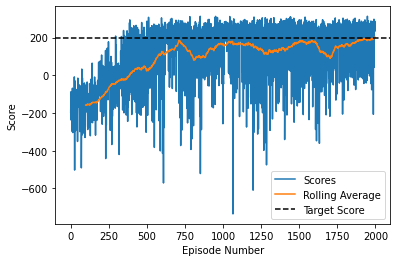
\includegraphics[width=\textwidth]{Deep Q Network Lunar Lander.png}
    \caption{Deep Q Network}
  \end{minipage}
  \hfill
  \begin{minipage}[b]{0.4\textwidth}
    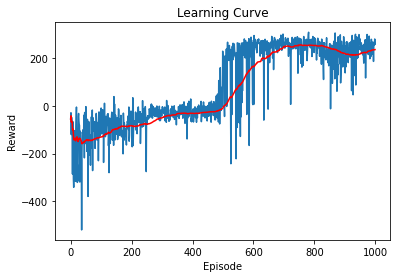
\includegraphics[width=\textwidth]{Double Deep Q Network Lunar Lander.png}
    \caption{Double Deep Q Network}
  \end{minipage}
\end{figure}
\\
In the game of \textit{CartPole}:
\begin{figure}[h!]
  \centering
  \begin{minipage}[b]{0.4\textwidth}
    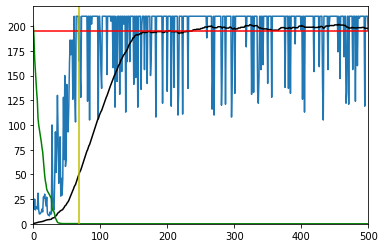
\includegraphics[width=\textwidth]{Deep Q Network CartPole.png}
    \caption{Deep Q Network}
  \end{minipage}
  \hfill
  \begin{minipage}[b]{0.4\textwidth}
    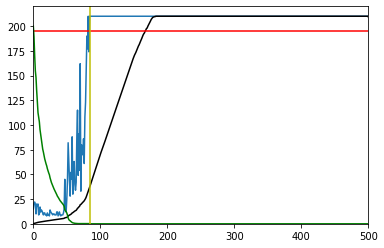
\includegraphics[width=\textwidth]{Double DQN Cartpole.png}
    \caption{Double Deep Q Network}
  \end{minipage}
\end{figure}

\section{Summary}
In this report, we have discussed about the theoretical and mathematical base of Deep Q Network and Double Deep Q Network, which are among the most important base of Reinforcement Learning. We then visualize to compare performance between DQN and DDQN.
\newpage
\medskip
\bibliography{ref}
\end{document}
